\begin{recipe}
    [% 
        preparationtime = {\unit[25]{min}},
        bakingtime = {\unit[45]{min}},
        portion = {one good party},
        source = {kwestiasmaku.com: lesny-mech}
    ]
    {The forest moss cake}

    \introduction{%
        Fear not, you won't be able to sense the taste of the spinach (partly because it doesn't have much taste anyway); I've tested that on my family.
    }

    \ingredients{%
        & pomegranate \textbf{and/or} \\
        & blueberries \\
        & fresh mint \\
        & \textbf{Cake} \\
        \unit[450]{g} & spinach \\
        \unit[\nicefrac{1}{2}]{c.} & oil \\
        \unit[\nicefrac{1}{2}]{c.} & sugar \\
        3 & eggs \\
        \unit[2]{c.} & flour \\
        \unit[2]{ts.} & baking powder \\
        & \textbf{Cream} \\
        \unit[250]{g} & mascarpone \\
        \unit[200]{ml} & crème fraîche/double cream \\
        & icing sugar  
    }

    \preparation{%
        \step Defrost spinach if needed, blend into a uniform paste.
        If you have fresh spinach, heat it up for 3 minutes on a pan first.

        \step Preheat the oven to \unit[180]{\textcelcius}. Crack the eggs into a bowl, add sugar and beat.
        Continue beating while slowly pouring in the oil.
        Add the spinach and blend (low power) until the two ingredients mix.

        \step Mix the flour with baking powder, add to the mixture and briefly blend again.
        Pour the mix into a round form and bake for \unit[40-45]{minutes} until dry inside.
        Take out and cool down to room temperature.

        \step Beat all the cream ingredients until stiff.

        \step Cut off the top third of the cake.
        Spread the cream on the bottom part.
        Break the top into small crumbs and use them to decorate the cream.
        Decorate with fruit and basil leafs.
    }

    \hint{%
        Reportedly beating the eggs is easier if they are warm.
        Put them into hot tap water for 10 minutes.
    }

\end{recipe}


\begin{figure}[h]
    \centering
    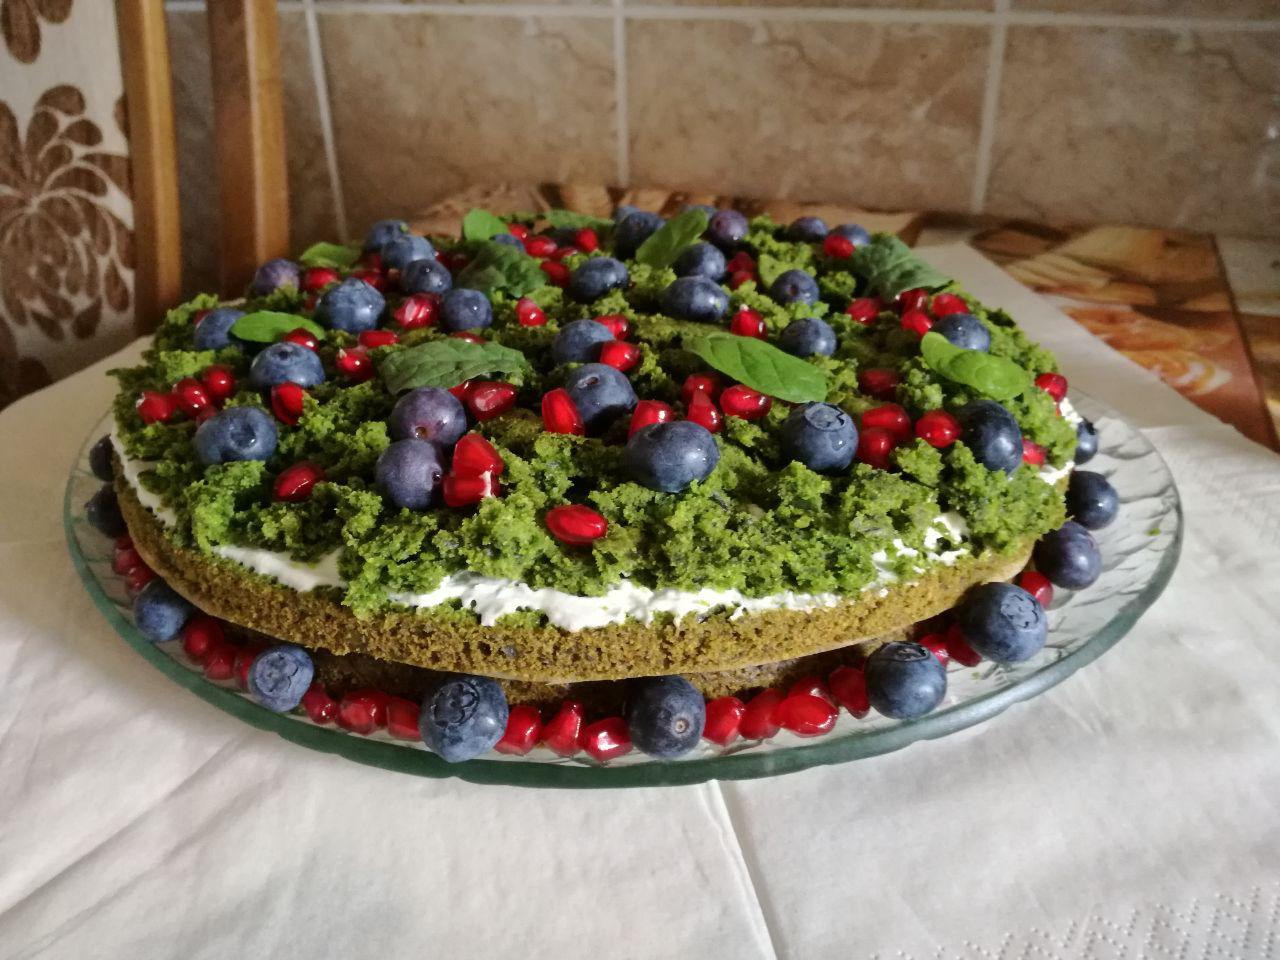
\includegraphics[width=12cm]{pic/forest_moss}
\end{figure}
\begin{figure}[h]
    \centering
    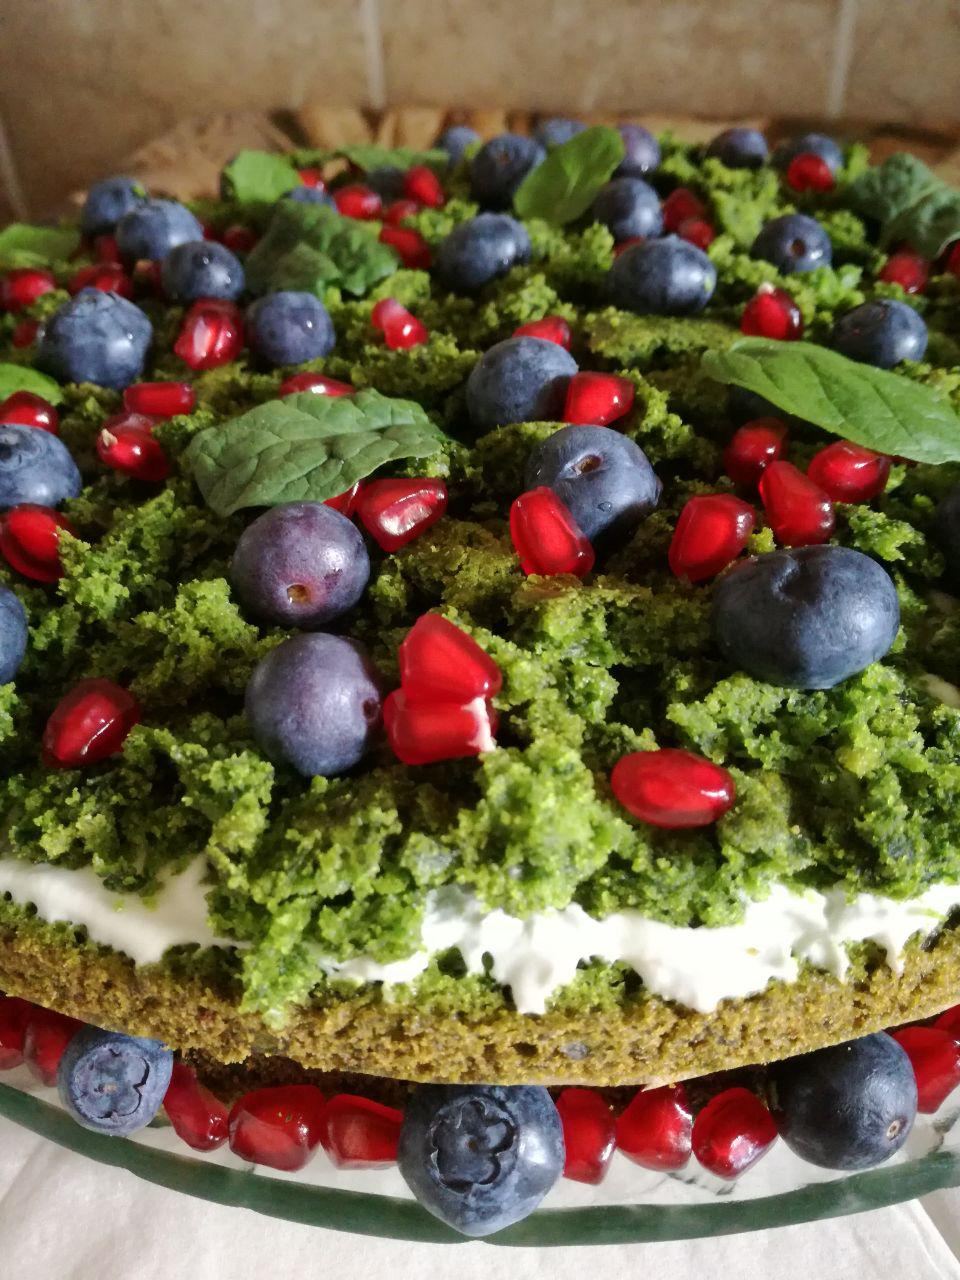
\includegraphics[width=10cm]{pic/forest_moss_2}
\end{figure}
